\documentclass[tikz,border=5pt]{standalone}
\usepackage{amsmath, amssymb} % 수식용 패키지
\usetikzlibrary{arrows.meta, positioning, bending, calc, decorations.pathmorphing}

% --- 색상 정의 (그림과 유사하게) ---
\definecolor{myTeal}{RGB}{0, 153, 153}
\definecolor{myOrange}{RGB}{204, 102, 51}
\definecolor{myPurple}{RGB}{128, 102, 153}
\definecolor{myDarkGrey}{RGB}{80, 80, 80}

\begin{document}

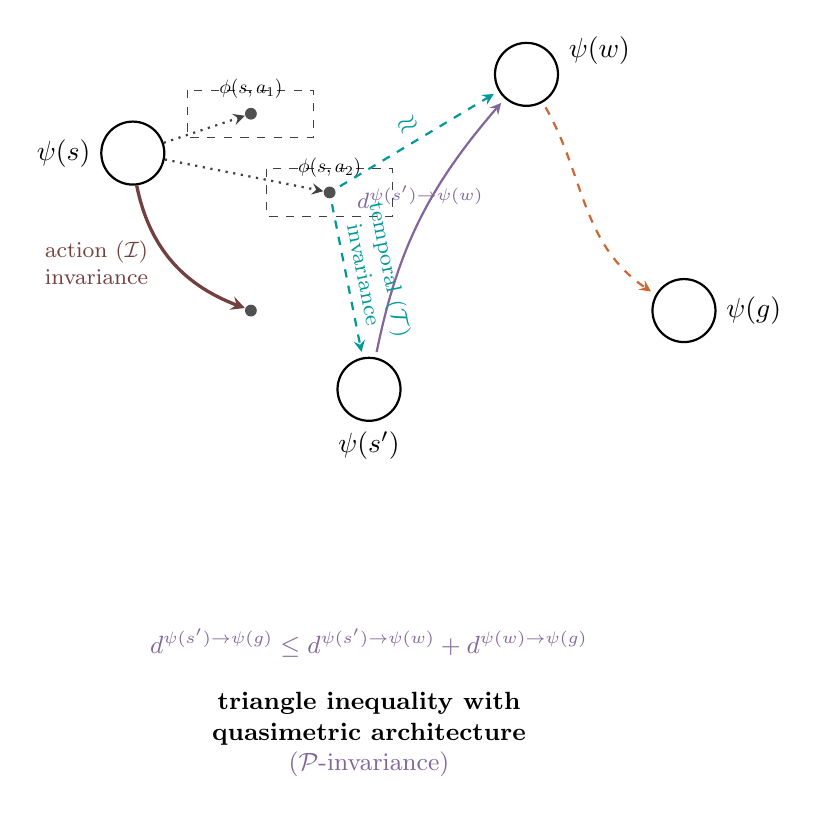
\begin{tikzpicture}[
    % --- 스타일 정의 (여기가 핵심!) ---
    % 1. 노드 스타일
    mainnode/.style={circle, draw=black, thick, minimum size=0.8cm, inner sep=1pt, font=\small},
    smallnode/.style={circle, fill=myDarkGrey, minimum size=0.15cm, inner sep=0pt},
    % 2. 화살표 스타일
    stdarrow/.style={->, >=stealth, thick}, % 기본 화살표
    teal-dashed/.style={stdarrow, myTeal, dashed, shorten >=2pt, shorten <=2pt}, % 청록색 점선
    orange-dashed/.style={stdarrow, myOrange, dashed, shorten >=2pt, shorten <=2pt}, % 주황색 점선
    purple-arrow/.style={stdarrow, myPurple, shorten >=2pt, shorten <=2pt}, % 보라색 실선
    action-arrow/.style={->, >=stealth, very thick, myDarkGrey!80!red}, % 빨간색 액션 화살표
    % 3. 텍스트 라벨 스타일
    labeltext/.style={font=\footnotesize, align=center}
]

% === 1단계: 노드(점) 배치 ===
% 좌표를 찍어서 대략적인 위치를 잡습니다.
\node[mainnode] (psi_s) at (0, 3) {}; \node[left] at (psi_s.west) {$\psi(s)$};
\node[mainnode] (psi_sp) at (3, 0) {}; \node[below] at (psi_sp.south) {$\psi(s')$};
\node[mainnode] (psi_w) at (5, 4) {}; \node[above right] at (psi_w.east) {$\psi(w)$};

% 작은 회색 점들 배치 (상대 위치 활용)
\node[smallnode] (s_a1) at ($(psi_s)+(1.5, 0.5)$) {};
\node[smallnode] (s_a2) at ($(psi_s)+(2.5, -0.5)$) {};
\node[smallnode] (s_a3) at ($(psi_s)+(1.5, -2)$) {};


% === 2단계: 화살표 그리기 ===
% --- (s) 주변의 작은 점선 박스와 화살표 ---
\draw[dashed, thin, darkgray] ($(s_a1)+(-0.8,0.3)$) rectangle ($(s_a1)+(0.8,-0.3)$);
\node[scale=0.7] at (s_a1) [above=3pt] {$\phi(s,a_1)$};
\draw[stdarrow, darkgray, dotted] (psi_s) -- (s_a1);

\draw[dashed, thin, darkgray] ($(s_a2)+(-0.8,0.3)$) rectangle ($(s_a2)+(0.8,-0.3)$);
\node[scale=0.7] at (s_a2) [above=3pt] {$\phi(s,a_2)$};
\draw[stdarrow, darkgray, dotted] (psi_s) -- (s_a2);

% 빨간색 액션 화살표 (구부리기: bend right)
\draw[action-arrow] (psi_s) to[bend right=30] node[left, labeltext, xshift=-5pt] {action ($\mathcal{I}$)\\invariance} (s_a3);


% --- 메인 삼각형 화살표 ---
% 1. 보라색 (s' -> g) : 살짝 구부림 (bend left)
\draw[purple-arrow] (psi_sp) to[bend left=15] coordinate[midway](mid_purple) (psi_w);
% 화살표 위에 수식 올리기 (sloped: 기울기에 맞춤)
\node[labeltext, myPurple, above, sloped] at (mid_purple) {$d^{\psi(s') \to \psi(w)}$};


% 2. 청록색 점선 (s -> s', s -> w)
\draw[teal-dashed] (s_a2) -- node[midway, above, sloped, labeltext] {temporal ($\mathcal{T}$)\\invariance} (psi_sp);
\draw[teal-dashed] (s_a2) -- node[midway, above, sloped, font=\bfseries] {$\approx$} (psi_w);

% 3. 주황색 점선 (w -> g)
% 많이 구부려야 할 때는 to[out=각도, in=각도]를 씁니다.
\node[mainnode] (psi_g) at (7, 1) {}; \node[right] at (psi_g.east) {$\psi(g)$};
\draw[orange-dashed] (psi_w) to[out=-60, in=150] (psi_g);


% === 3단계: 하단 텍스트 ===
\node[below=2.5cm of psi_sp, align=center, font=\small] {
\textcolor{myPurple}{$d^{\psi(s') \to \psi(g)} \le d^{\psi(s') \to \psi(w)} + d^{\psi(w) \to \psi(g)}$} \\[1em]
\textbf{triangle inequality with} \\
\textbf{quasimetric architecture} \\
\textcolor{myPurple}{($\mathcal{P}$-invariance)}
};

\end{tikzpicture}
\end{document}